\section{Characterization} \label{sec:characterization}

In this section, the Omicron algorithm is characterized. To achieve this, we consider Gaussian noise and, on top of it, we inject sinusoidal Gaussian burst signals with known characteristics. This is done using the injection feature of Omicron described in Sec.~\ref{sec:algorithm:injections}. The burst waveform is given in Eq.~\ref{eq:sginj}. Then, we estimate the accuracy with which Omicron recovers the signal parameters.
\begin{itemize}
\item The timing accuracy is estimated with the absolute time difference, $\tau_o-\tau_b$, where $\tau_o$ is the time measured by Omicron (tile time) and $\tau_b$ is the time of the injection.
\item The frequency accuracy is estimated with the relative difference, $(\phi_o-\phi_b)/\phi_b$, where $\phi_o$ is the frequency measured by Omicron (tile frequency) and $\phi_b$ is the frequency of the injection.
\item The SNR accuracy is estimated with the relative difference, $(\rho_o-\rho_b)/\rho_b$, where $\rho_o$ is the SNR estimated by Omicron (tile SNR computed with Eq.~\ref{eq:snrestimator}) and $\rho_b$ is the SNR of the injection given by Eq.~\ref{eq:snr_white}.
\end{itemize}



\subsection{White noise} \label{sec:characterization:white}
As a first characterization test, we simulate burst signals on top of white noise. The injection frequency $\phi_b$ and quality factor $Q_b$ take random values between 32~Hz and 256~Hz and between 4 and 64 respectively. The time of the injection is randomly drawn in $\pm10$~s around the chunk center. Signals are injected using a fix amplitude $B$ such that the resulting SNR is $\rho_b=10$. Then we run Omicron with the parameters listed in Appx~\ref{appx:parameters} over a data set containing 1038 injections. The maximal fractional energy loss between tiles is varied around the nominal value of $\mu_{max}=20\%$ and the resulting recovery histograms for SNR, time and frequency are displayed in Fig.~\ref{fig:char_mismatch}. The SNR recovery histogram is well compatible with the Monte Carlo study presented in Fig.~\ref{fig:snrestimator} and Tab.~\ref{tab:snrestimator}. The mean value for the $\mu_{max}=5\%$ distribution is -0.8\% while it was predicted to be -0.51\% when the match between the tile and the signal is perfect. The standard deviation for $\mu_{max}=20\%$ is $\pm9.95\%$ while it was found to be $\pm10.08\%$ with Monte Carlo studies. The time and frequency recovery histograms are well centered on 0 proving that Omicron does not introduce any bias. Omicron adopts a multi-resolution tiling structure (see Sec.~\ref{sec:algorithm:tiling}): the time and frequency resolution is a function of the frequency and the quality factor. Fig.~\ref{fig:char_mismatch} show that, for the parameter ranges given above and for $\mu_{max}=20\%$, the timing is known at $\pm8$~ms and the frequency is resolved at $\pm2.4\%$. 
\begin{figure}
  \center
  \epsfig{width=8.5cm, file=./figures/char_mismatch_snr.eps}
  \epsfig{width=8.5cm, file=./figures/char_mismatch_time.eps} \\
  \epsfig{width=8.5cm, file=./figures/char_mismatch_freq.eps}
  \caption{Omicron SNR, time and frequency reconstruction performance as a function of the maximal fractional energy loss between tiles, $\mu_{max}$. Four values of $\mu_{max}$ were used: 5\% (blue), 10\% (black), 20\% (red) and 30\% (green). The distribution mean values and standard deviations are reported in the color boxes.}
  \label{fig:char_mismatch}
\end{figure}

Now, we fix the $\mu_{max}$ parameter to 20\% and we choose discrete values for the quality factor of the injections: $Q_b=4$, $Q_b=16$, $Q_b=32$ and $Q_b=64$. Fig.~\ref{fig:char_q} shows how Omicron recovers the signal parameters for these four data sets.
\begin{figure}
  \center
  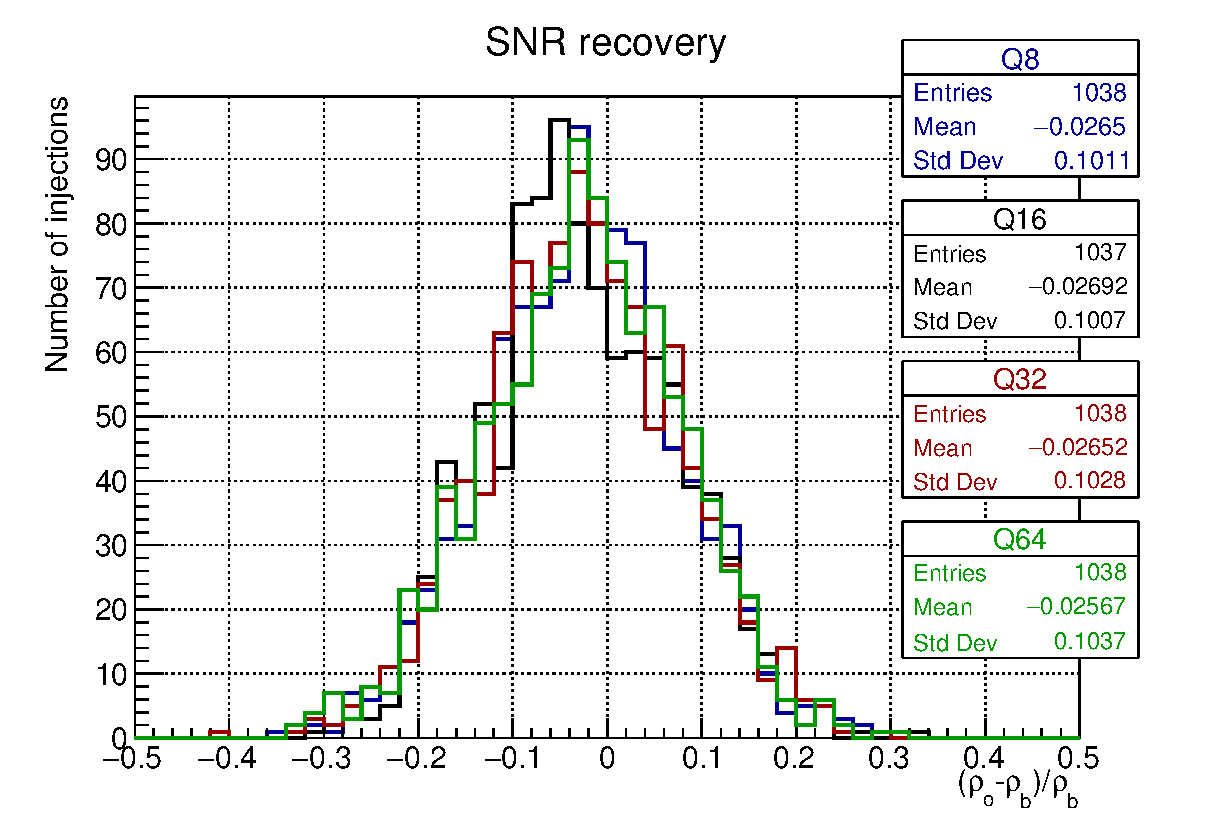
\epsfig{width=8.5cm, file=./figures/char_Q_snr.eps}
  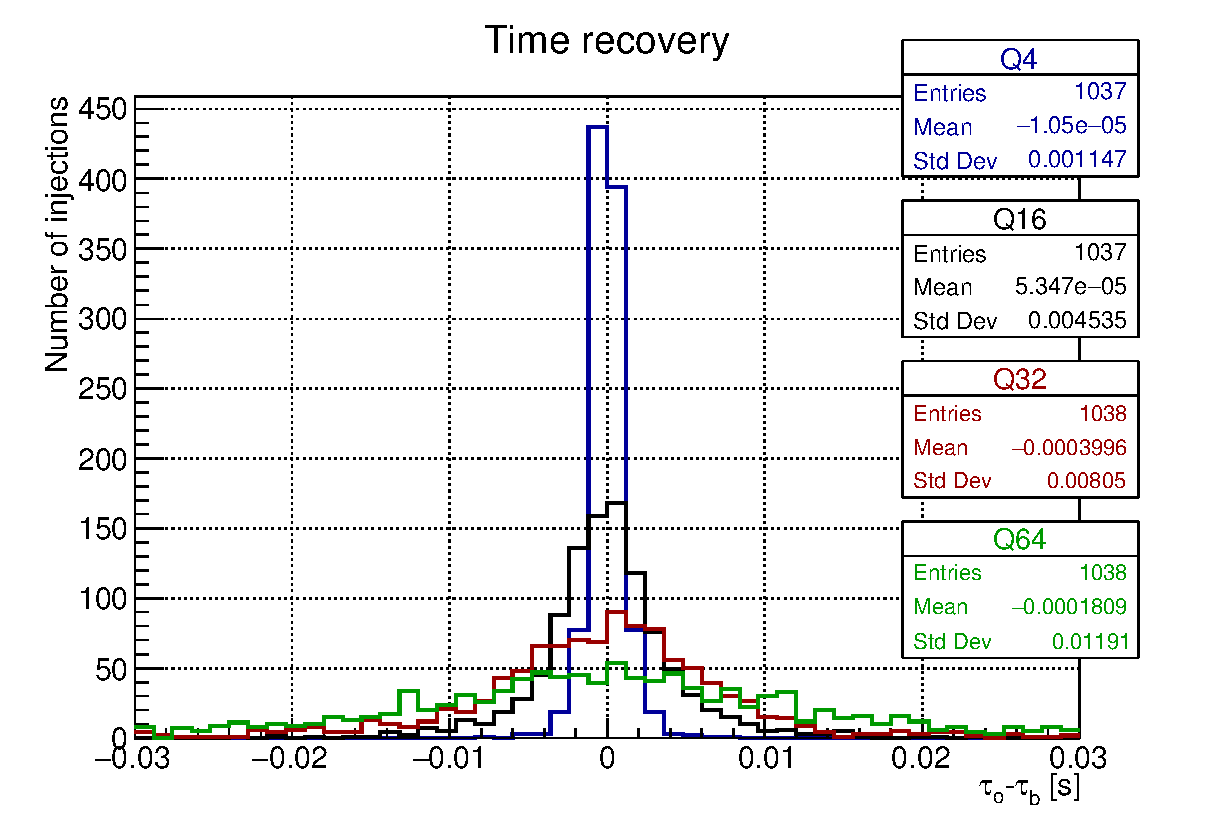
\epsfig{width=8.5cm, file=./figures/char_Q_time.eps} \\
  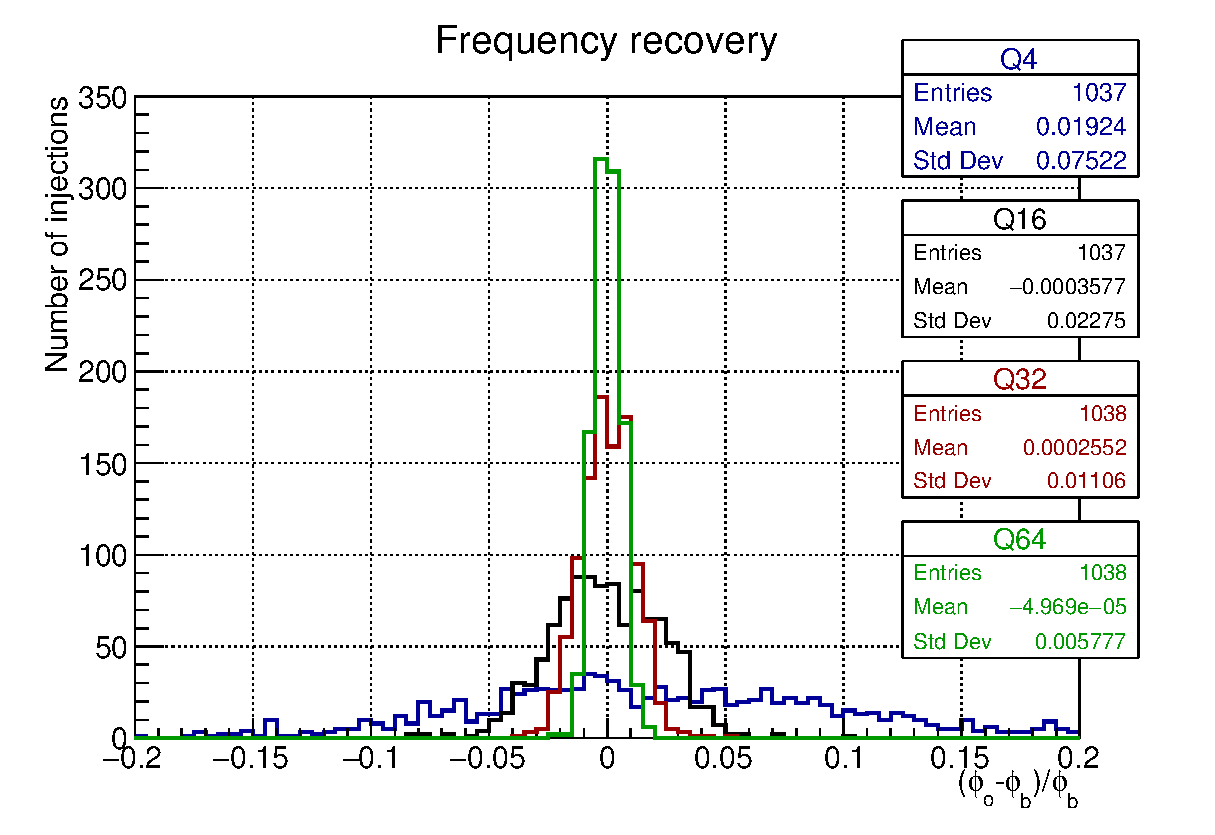
\epsfig{width=8.5cm, file=./figures/char_Q_freq.eps}
  \caption{Omicron SNR, time and frequency reconstruction performance as a function of the signal quality factor, $Q_b$. Four values of $Q_b$ were used: 4 (blue), 16 (black), 32 (red) and 64 (green). The distribution mean values and standard deviations are reported in the color boxes.}
  \label{fig:char_q}
\end{figure}


\subsection{Colored noise} \label{sec:characterization:colored}

the amplitude spectral density of which is represented in Fig.~\ref{fig:noise_asd}. On top of this, sinusoidal Gaussian burst signals are injected. The signal expression is given by 
\begin{figure}
  \center
  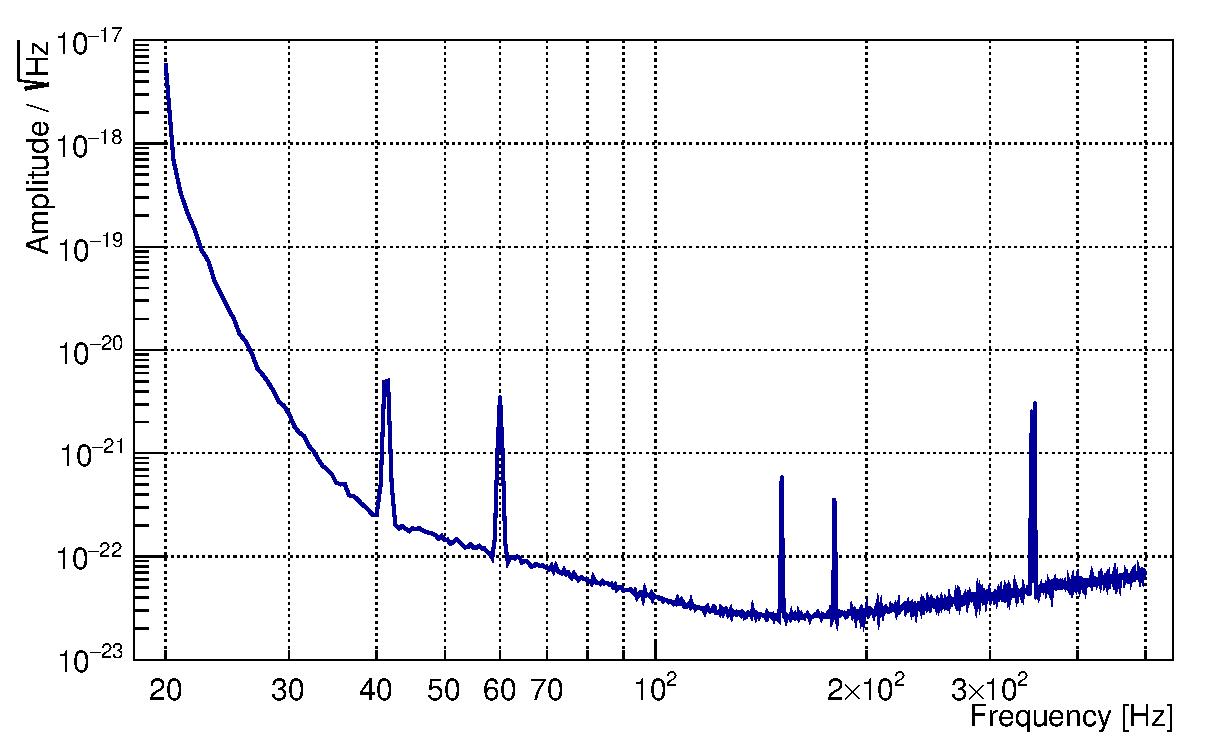
\epsfig{width=10cm, file=./figures/noise_asd.eps}
  \caption{Noise spectral density}
  \label{fig:noise_asd}
\end{figure}
